\documentclass[12pt]{article}
\usepackage{amsmath,amssymb}
\usepackage{mathtools}
\usepackage{hyperref}

\usepackage{tikz}
\usepackage{cancel}

\usepackage{siunitx}
\sisetup{per-mode=fraction,group-digits=none}

\usetikzlibrary{decorations.pathreplacing}

\title{Approximating the Period of a Pendulum\\[0.2em]
\large AP Calculus BC: Taylor Series Project}
\author{Andrew Chou \and Kevin Ma \and James Tsaggaris}

\linespread{1.25}
\setlength{\skip\footins}{3\baselineskip}   % Adjust space between
% text and footnotes

\begin{document}

\maketitle

\begin{center}
  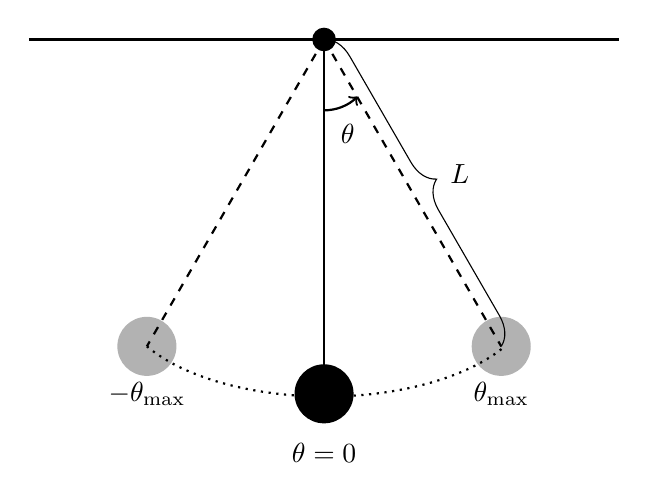
\begin{tikzpicture}[scale=1.5]
    % Draw ceiling
    \draw[thick] (-2.5,3) -- (2.5,3);

    % Draw pivot point
    \fill[black] (0,3) circle (0.1);

    % Calculate pendulum length (3 units)
    \def\pendulumLength{3}

    % Draw pendulum at equilibrium position (vertical)
    \draw[thick] (0,3) -- (0,{3-\pendulumLength});
    \fill[black] (0,{3-\pendulumLength}) circle (0.25);

    % Draw left swing position (30 degrees)
    \draw[thick,dashed] (0,3) --
    ({-\pendulumLength*sin(30)},{3-\pendulumLength*cos(30)});
    \fill[black,opacity=0.3]
    ({-\pendulumLength*sin(30)},{3-\pendulumLength*cos(30)}) circle (0.25);

    % Draw right swing position (30 degrees)
    \draw[thick,dashed] (0,3) --
    ({\pendulumLength*sin(30)},{3-\pendulumLength*cos(30)});
    \fill[black,opacity=0.3]
    ({\pendulumLength*sin(30)},{3-\pendulumLength*cos(30)}) circle (0.25);

    % Draw connecting arc for the path
    \draw[thick,dotted]
    ({-\pendulumLength*sin(30)},{3-\pendulumLength*cos(30)}) arc
    (-150:-30:1.75 and 0.85);

    % Draw angle theta (to right swing position)
    \draw[->,thick] (0,2.4) arc (-90:-45:0.4);
    \node at (0.2,2.2) {$\theta$};

    % Label theta max at the right swing position
    \node at (1.5,0) {$\theta_{\mathrm{max}}$};

    % Label negative theta max at the left swing position
    \node at (-1.5,0) {$-\theta_{\mathrm{max}}$};

    % Label equilibrium position
    \node at (0,-0.5) {$\theta = 0$};

    % Oblique overbrace representing L for the right pendulum
    \draw[decorate,decoration={brace,amplitude=10pt}] (0,3) --
    ({\pendulumLength*sin(30)},{3-\pendulumLength*cos(30)})
    node[midway,above,xshift=17pt] {$L$};
  \end{tikzpicture}
\end{center}

\section{Inputs}
\begin{itemize}
  \item $L$: Length of pendulum (meters)
  \item $\theta_{\mathrm{max}}$: Maximum angular displacement (radians)
\end{itemize}

\section{Period of a Pendulum}
\[
  T = 4 \sqrt{\frac{L}{g}} \int_{0}^{\frac{\pi}{2}} \frac{1}{\sqrt{1 - k^2
  \sin^2 \theta}} \, d\theta
\]
where $k = \sin\left(\frac{\theta_{\mathrm{max}}}{2}\right)$ (a constant).

\section{Series Expansion}
Let $u = k^2 \sin^2 \theta$, and the integrand becomes:
\[
  f(u) = \frac{1}{\sqrt{1 - u}} = (1 - u)^{-\frac{1}{2}}
\]
which is in the form of a binomial series $(1+x)^k =
\sum_{n=0}^{\infty} \binom{k}{n} x^n$.

Since we have not yet covered binomial series in class, we will instead
use the Maclaurin series expansion for $(1 - u)^{-1/2}$ around $u =
0$. First, we find the general form of the $n$th derivative:
\begin{align*}
  f^{(0)}(u) &= (1-u)^{-\frac{1}{2}} &&\rightarrow f^{(0)}(0) =
  \frac{1}{\cancel{2^0}} \\
  f^{(1)}(u) &= -\frac{1}{2} (1-u)^{-\frac{3}{2}} (-1) &&\rightarrow
  f^{(1)}(0) = \frac{1}{2^1} \\
  f^{(2)}(u) &= -\frac{1\cdot3}{2^2} (1-u)^{-\frac{5}{2}} (-1)
  &&\rightarrow f^{(2)}(0) = \frac{1\cdot3}{2^2} \\
  f^{(3)}(u) &=
  -\frac{\color{blue}\overbrace{1\cdot3\cdot5}^{\mathclap{\text{odd-only
  factorial}}}}{\color{red}2^3} (1-u)^{\color{orange} -\frac{7}{2}} (-1)
  &&\rightarrow f^{(3)}(0) =
  \frac{1\cdot3\cdot5}{2^3} \\
  f^{(n)}(u) &= \frac{{\color{blue}(2n-1)!!}}{{\color{red}2^n}}
  (1-u)^{\color{orange} -\frac{2n+1}{2}}
  &&\rightarrow f^{(n)}(0) = \frac{{(2n-1)!!}}{{2^n}}
\end{align*}

Plugging in to the Maclaurin series formula $f(x) =
\sum_{n=0}^{\infty} \frac{f^{(n)}(0)}{n!} x^n$, we get:
\[
  \frac{1}{\sqrt{1 - u}} = \sum_{n=0}^{\infty} \frac{
  (2n-1)!!}{2^n n!} u^n
\]
Since $2^n n!$ is equivalent to multiplying by 2 for every term in
the factorial, we can rewrite the series as the following, after
substituting $u = k^2 \sin^2 \theta = (k\sin\theta)^2$:
\[
  \sum_{n=0}^{\infty} \frac{(2n-1)!!}{(2n)!!}
  {\left(k\sin\theta\right)}^{2n}
\]
Keep in mind that for $n = 0$, $(2(0) - 1)!! = (-1)!! = 1$ by
convention. \footnote{\url{https://mathworld.wolfram.com/DoubleFactorial.html}}

\section{Simplifying the Integral}

Substitute the above Maclaurin series into the integral:
\[
  \int_{0}^{\frac{\pi}{2}} \frac{1}{\sqrt{1 - k^2
  \sin^2 \theta}} \, d\theta = \int_{0}^{\frac{\pi}{2}}
  \sum_{n=0}^{\infty} \left[\frac{(2n-1)!!}{(2n)!!}
  {\left(k\sin\theta\right)}^{2n}\right] \, d\theta
\]
Take constant (non-$\theta$) terms out of the integral, since they
are independent of $\theta$:
\[
  = \sum_{n=0}^{\infty} \left[\frac{(2n-1)!!}{(2n)!!} k^{2n}
  \int_{0}^{\frac{\pi}{2}} \sin^{2n} \theta \, d\theta\right]
\]

We evaluate the first three terms of the series to get a sense of the pattern:
\[
  1 + \frac{1}{2}k^2\int_{0}^{\frac{\pi}{2}} \sin^2 \theta \, d\theta
  + \frac{3}{8}k^4\int_{0}^{\frac{\pi}{2}} \sin^4 \theta \, d\theta + \cdots
\]

Find the values of the definite integrals using half-angle identities:
\[
  \int_{0}^{\frac{\pi}{2}} \left(\frac{1}{2} -
  \frac{1}{2}\cos(2\theta)\right) \, d\theta = \left[\frac{\theta}{2}
  - \frac{1}{4}\sin(2\theta)\right]_{0}^{\frac{\pi}{2}} = \frac{\pi}{4}
\]
\[
  \int_{0}^{\frac{\pi}{2}} \sin^4 \theta \, d\theta =
  \left[\frac{\theta}{4} - \frac{1}{4}\sin(2\theta) +
    \frac{\theta}{8} +
  \frac{1}{32}\sin(4\theta)\right]_{0}^{\frac{\pi}{2}} =
  \frac{\pi}{8} + \frac{\pi}{16} = \frac{3\pi}{16}
\]

The resulting terms are:
\[
  1 + \frac{1}{2}k^2\left(\frac{\pi}{4}\right) +
  \frac{3}{8}k^4\left(\frac{3\pi}{16}\right) + \cdots
\]

The process is tedious, but we see that each integral is in the form
of Wallis integrals, defined by the sequence $W_n =
\int_{0}^{\frac{\pi}{2}} \sin^n \theta \, d\theta$. Evaluating each
definite integral gives some multiple of $\frac{\pi}{2}$, and the
antiderivative of all the recursive cosines from the half-angle
identities all vanish, since $\sin(2n \cdot \frac{\pi}{2}) =
\sin(n\pi) = 0$. Through integration by parts and recursive
substitution of $I$, the value of even Wallis integrals are known to be:
\[
  W_{2n} = \frac{(2n-1)!!}{(2n)!!} \cdot \frac{\pi}{2}
\]

After substituting in the value of the Wallis integrals, we can now
express the general (approximate) formula for the period of a
pendulum using the integrated Maclaurin series:
\begin{align*}
  T &= 4 \sqrt{\frac{L}{g}} \sum_{n=0}^{\infty} \left[\frac{
  (2n-1)!!}{(2n)!!} k^{2n} \cdot W_{2n}\right] \\
  &= 4 \sqrt{\frac{L}{g}} \sum_{n=0}^{\infty} \left[\frac{
    (2n-1)!!}{(2n)!!} k^{2n} \cdot \frac{(2n-1)!!}{(2n)!!} \cdot
  \frac{\pi}{2}\right] \\
  &= 4 \cdot \frac{\pi}{2} \sqrt{\frac{L}{g}} \sum_{n=0}^{\infty}
  \left[ k^{2n} \left(\frac{(2n-1)!!}{(2n)!!}\right)^2 \right] \\
  &= 2\pi \sqrt{\frac{L}{g}} \sum_{n=0}^{\infty} \left[
  \left(\frac{(2n-1)!!}{(2n)!!}\right)^2 k^{2n} \right]
\end{align*}

\section{Results}

Let $L = 1$ m and $\theta_{\mathrm{max}} = \frac{\pi}{6}$ radians. It follows that $k = \sin\left(\frac{\theta_{\mathrm{max}}}{2}\right) = \sin\left(\frac{\pi}{12}\right)$. The CIPM defines $g = \SI{9.80665}{\meter/\second\squared}$.

Using a calculator, the exact period of the pendulum is:
% https://www.wolframcloud.com/obj/662d9cb9-443c-46df-802f-d61b0c882544
\[
  T = 4\sqrt{\frac{1}{g}} \int_{0}^{\frac{\pi}{2}} \frac{1}{\sqrt{1 - \sin^2\left(\frac{\pi}{12}\right) \sin^2 \theta}} \, d\theta \approx \boxed{\SI{2.041339}{\second}}
\]

\begin{align*}
  T_0 &= 2\pi \sqrt{\frac{L}{g}} \left(1\right) \approx \boxed{\SI{2.006409}{\second}} \\
  T_1 &= 2\pi \sqrt{\frac{L}{g}} \left(1 + \frac{1}{4}k^2\right) \approx \boxed{\SI{2.040010}{\second}} \\
  T_2 &= 2\pi \sqrt{\frac{L}{g}} \left(1 + \frac{1}{4}k^2 + \frac{9}{64}k^4\right) \approx \boxed{\SI{2.041276}{\second}} \\
  T_3 &= 2\pi \sqrt{\frac{L}{g}} \left(1 + \frac{1}{4}k^2 + \frac{9}{64}k^4 + \frac{25}{256}k^6\right) \approx \boxed{\SI{2.041335}{\second}}
\end{align*}

As the number of terms approaches infinity, the value of $T$ converges to the value using the definite integral.
\[
  T = 2\pi \sqrt{\frac{L}{g}} \left(1 + \frac{1}{4}k^2 + \frac{9}{64}k^4 + \frac{25}{256}k^6 + \cdots\right)
\]


\section{Error Bound}

Using the ratio test,
\begin{align*}
  \lim_{n \to \infty} \left|\frac{a_{n+1}}{a_n}\right| &= \lim_{n \to \infty} \left|\frac{\left(\frac{(2n+1)!!}{(2n+2)!!}\right)^2 k^{2n+2}}{\left(\frac{(2n-1)!!}{(2n)!!}\right)^2 k^{2n}}\right| \\
  &= \lim_{n \to \infty} \left|\frac{\left(\frac{(2n+1)\cancel{(2n-1)!!}}{(2n+2)\cancel{(2n)!!}}\right)^2 \cancel{k^{2n}}k^2}{\left(\frac{\cancel{(2n-1)!!}}{\cancel{(2n)!!}}\right)^2 \cancel{k^{2n}}}\right| \\
  &= \lim_{n \to \infty} \left|\frac{(2n+1)^2}{(2n+2)^2} k^2\right| = \left|k^2\right| \tag{\text{ladder of functions}} \\
  &\implies \left|k^2\right| < 1 \implies -1 < k < 1 \implies -1 < \sin\left(\frac{\theta_{\mathrm{max}}}{2}\right) < 1 \\
  &\implies 0 < \theta_{\mathrm{max}} < \pi \tag{\text{$\theta_{\mathrm{max}}$ is nonnegative}}
\end{align*}

% SKIP THIS (OUT OF CLASS SCOPE)

% Test the right endpoint of the interval ($k = 1$):

% \[
%   (2n-1)!! = \frac{\overbrace{(2n)!}^{\mathclap{\text{odd and even factorials}}} }{\underbrace{(2n)!!}_{\mathclap{\text{even-only factorial}}}} = \frac{(2n)!}{2^n n!}
% \]

% \[
%   \sum_{n=0}^{\infty} \left(\frac{(2n-1)!!}{(2n)!!}\right)^2 = \sum_{n=0}^{\infty} \frac{\frac{(2n)!}{2^n n!}}{2^n n!} = \sum_{n=0}^{\infty} \frac{(2n)!}{(2^n n!)^2} 
% \]
% Ratio test (inconclusive):
% \[
%   \lim_{n \to \infty} \left|\frac{a_{n+1}}{a_n}\right| = \lim_{n \to \infty} \left|\frac{\frac{(2n+2)(2n+1)(2n)!}{(2^{n}\cdot2 \cdot (n+1)(n)!)^2}}{\frac{(2n)!}{(2^n n!)^2}}\right| = \lim_{n \to \infty} \left|\frac{(2n+2)(2n+1)}{4(n+1)^2}\right| = 1
% \]

The maximum error bound is given by the next term in the series.
\[T_\infty = T_j + R_j \quad \implies \quad R_j = T_\infty - T_j \leq a_{j+1} \]
\begin{align*}
  T_0 \approx \SI{2.006409}{\second} \quad &\implies \quad R_0 \leq 2\pi \sqrt{\frac{L}{g}} \left(\frac{1}{4}k^2\right) \approx \boxed{\SI{0.001266}{\second}} \\
  T_1 \approx \SI{2.040010}{\second} \quad &\implies \quad R_1 \leq 2\pi \sqrt{\frac{L}{g}} \left(\frac{9}{64}k^4\right) \approx \boxed{\SI{0.000059}{\second}} \\
  T_2 \approx \SI{2.041276}{\second} \quad &\implies \quad R_2 \leq 2\pi \sqrt{\frac{L}{g}} \left(\frac{25}{256}k^6\right) \approx \boxed{\SI{0.000003}{\second}} \\
  T_3 \approx \SI{2.041335}{\second} \quad &\implies \quad R_3 \leq 2\pi \sqrt{\frac{L}{g}} \left(\frac{49}{1024}k^8\right) \approx \boxed{\SI{0.000000}{\second}} \\
\end{align*}

\end{document}
